\section{Task Formulation}
\label{sec:method}
In this section, we present Rex-Omni's task formulation design, covering its coordinate representation, the specific output formats for different tasks, and the details of its model architecture.
\subsection{Coordinate Formulation}

\begin{figure*}[t]
    \centering
    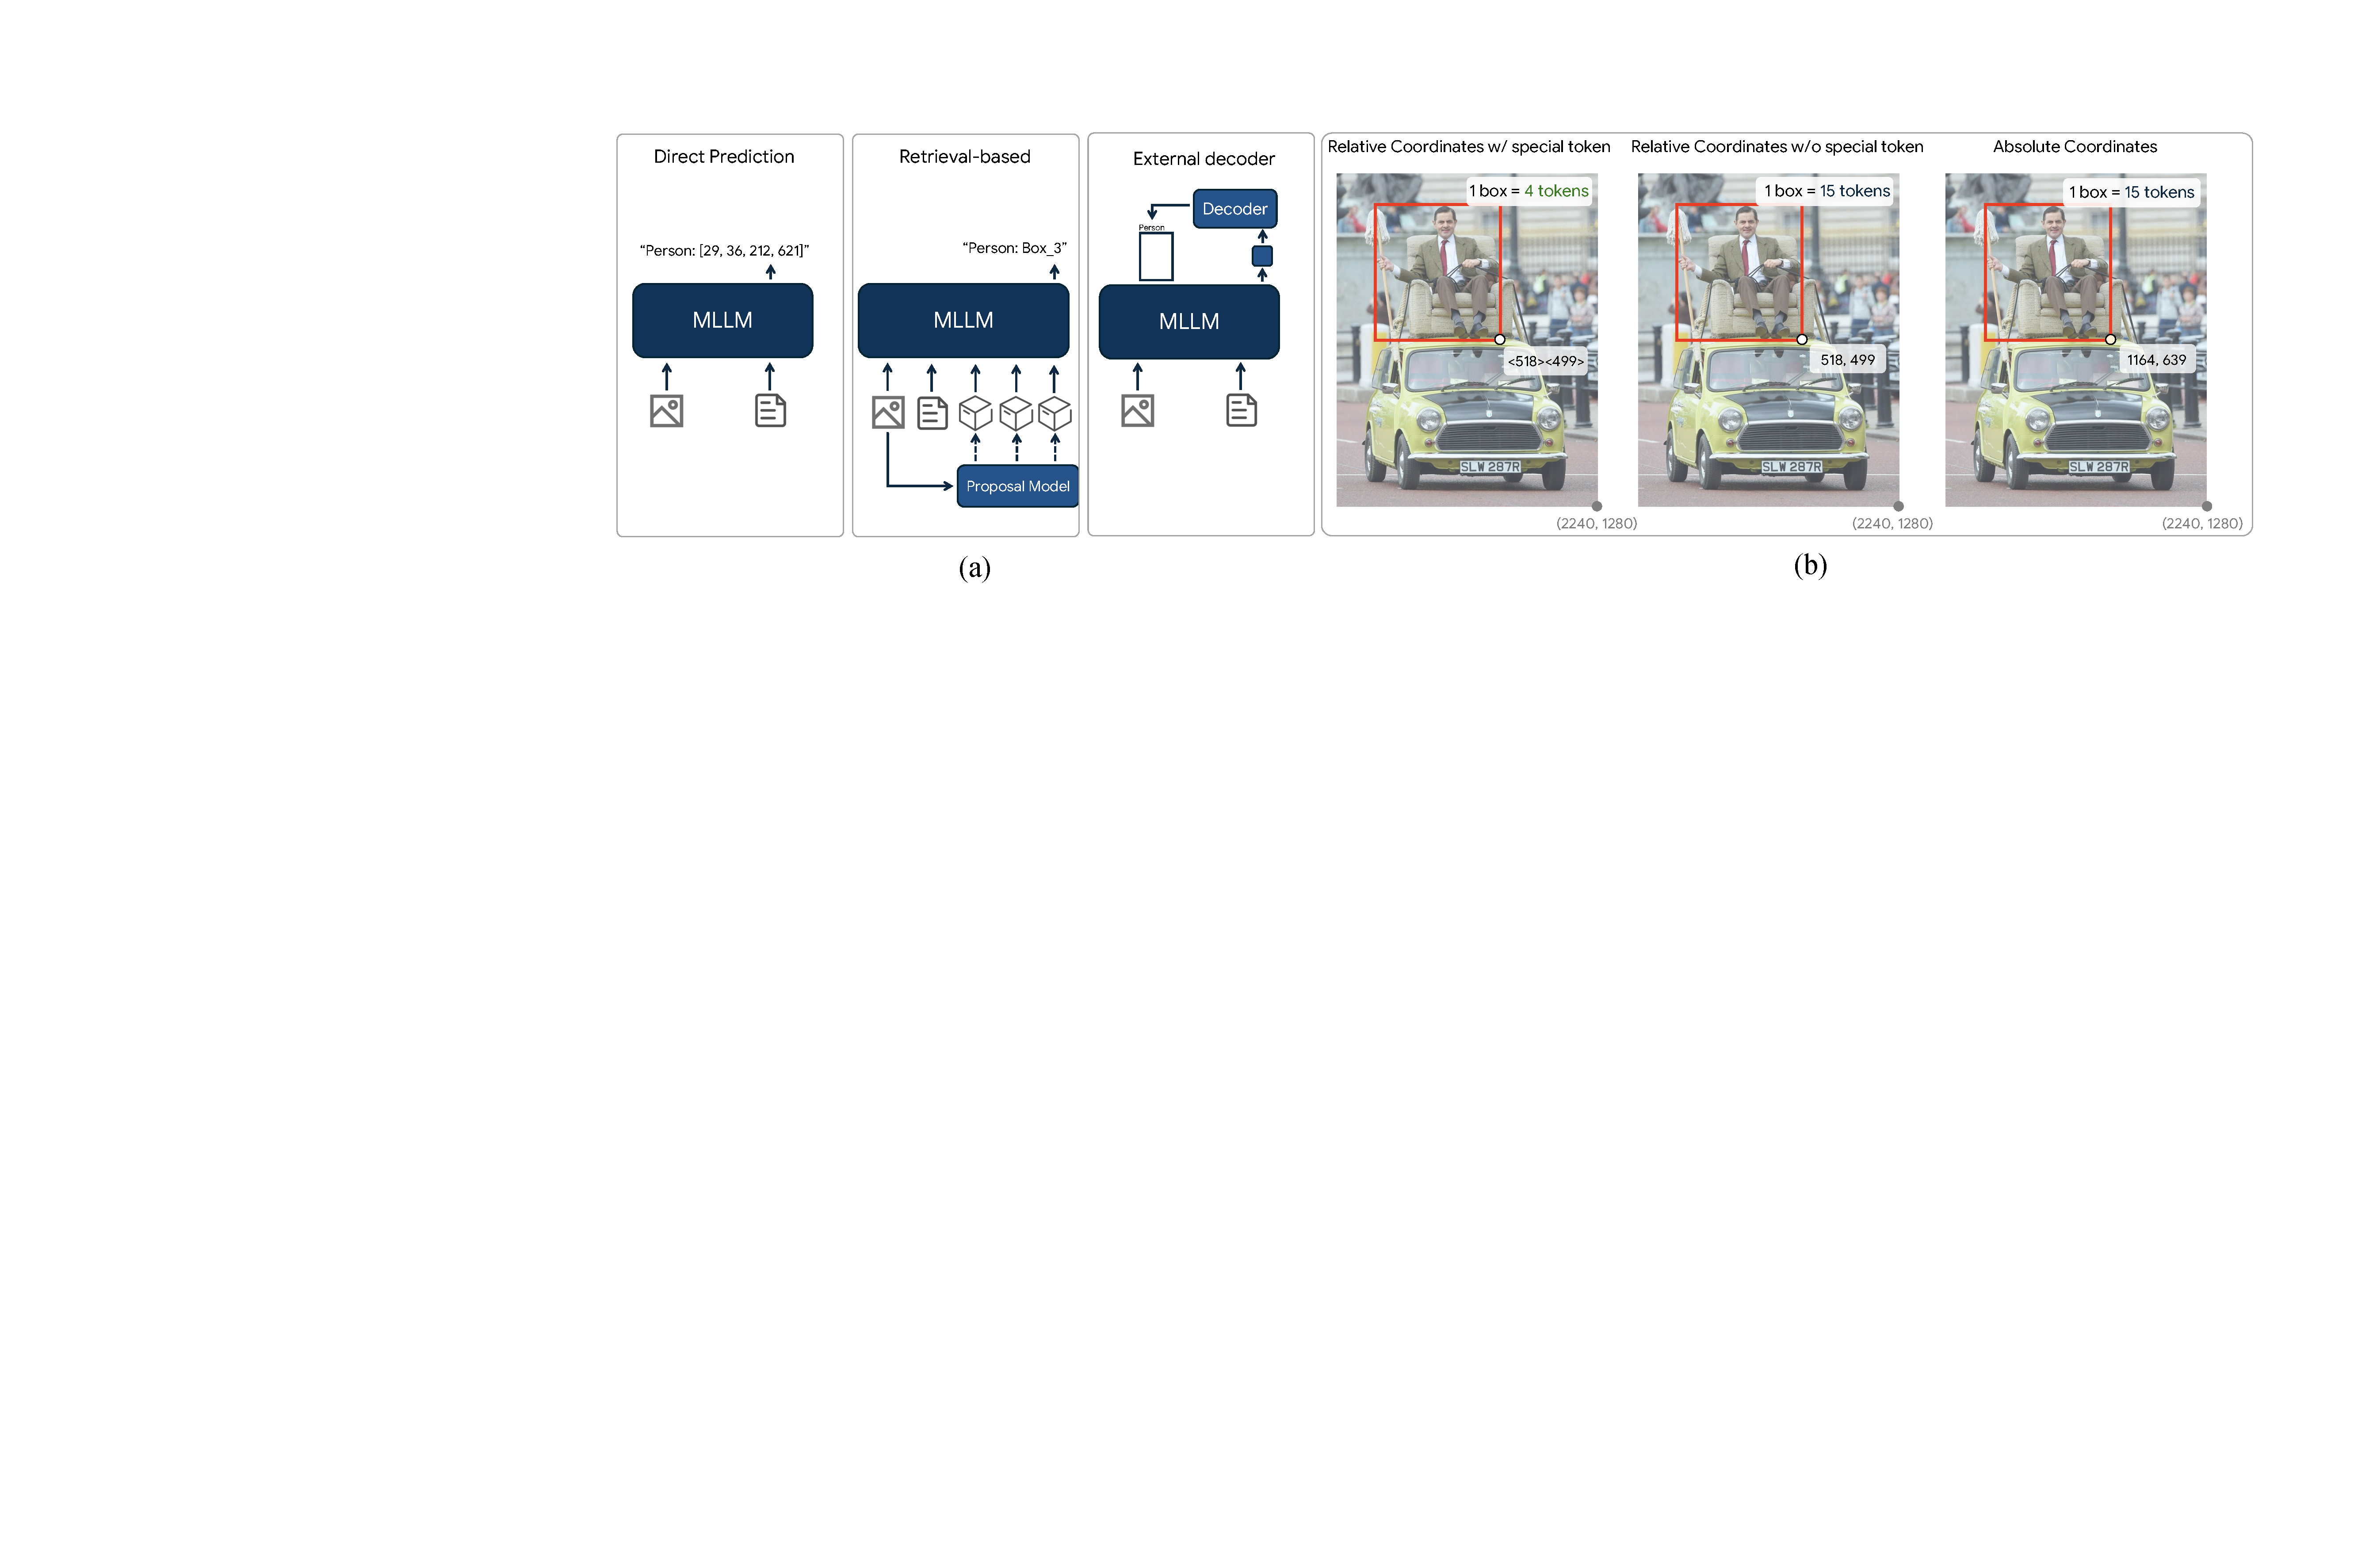
\includegraphics[width=\textwidth]{figures/task_design.pdf}
    \caption{Design philosophy of Rex-Omni for coordinate prediction. It illustrates our chosen approach: (a) adopting a direct coordinate prediction strategy, and (b) employing a quantized relative coordinate format represented by special tokens for efficient and robust spatial encoding.}
    \label{fig:philosophy}
\end{figure*}

We begin by defining the output formulation for coordinate prediction. Existing approaches to utilizing MLLMs for this task can be broadly categorized into three paradigms, as illustrated in Figure \ref{fig:philosophy}a: \textbf{1) Direct Coordinate Prediction:} Inspired by the Pix2Seq~\cite{chen2021pix2seq} paradigm, these method~\cite{chen2023shikra, you2023ferret, wang2023cogvlm, zhan2025griffon, zhang2024ferret} treats coordinate values as discrete tokens within the language model's vocabulary, enabling the model to directly generate coordinate outputs;
\textbf{2) Retrieval-based Methods:} This approach~\cite{jiang2024chatrex, ma2024groma, jiang2025rex, jiang2025referringperson} incorporates an additional proposal module. The LLM is trained to predict the index of a candidate region or bounding box, thereby representing the output as a retrieval task over predefined proposals;
\textbf{3) External decoder:} In this strategy~\cite{zhang2023nextchatlmmchatdetection, wu2024visionllm, lai2024lisa, liu2025seg}, the LLM predicts special tokens, whose corresponding embeddings are then passed to an external decoder responsible for producing the final coordinates. We adopt the direct coordinate prediction strategy for Rex-Omni, motivated by its simplicity, flexibility, and the advantage of not relying on external modules or additional supervision.

Within the direct coordinate prediction paradigm, several variations exist, as illustrated in Figure \ref{fig:philosophy}b:
\textbf{1) Relative coordinates with special tokens:} Coordinates are quantized to values between 0 and 999, with each coordinate represented by a special token in the LLM's vocabulary. The model is thus trained to predict these 1,000 tokens as representations for coordinates. A representative model is Pix2Seq~\cite{chen2021pix2seq}.
\textbf{2) Relative coordinates without special tokens:} Coordinates are similarly quantized to 1,000 bins; however, they are represented by multiple atomic tokens rather than a single special token. A representative model is SEED1.5-VL~\cite{guo2025seed1}.
\textbf{3) Absolute coordinates:} This method uses absolute coordinates, where a coordinate value such as 1921 is tokenized into individual digits (1, 9, 2, 1).  A representative model is Qwen2.5-VL~\cite{bai2025qwen2}. We choose relative coordinates with special tokens modeling approach for two primary reasons: First, selecting relative coordinates over absolute coordinates inherently reduces learning complexity by confining the classification task to a bounded range of 1,000 categories. Second, the use of dedicated special tokens for coordinates significantly reduces the required token length per coordinate. For instance, a bounding box is represented by only four special tokens, in contrast to 15 atomic tokens (including separators) without such a scheme. This significantly improves token efficiency and inference speed, especially in dense object scenes.

\subsection{Input Format}

Rex-Omni adopts a unified text-based interface for all visual perception tasks. Each task is expressed as a natural language query that specifies the target objects or relationships to be identified in the image. This design allows the model to seamlessly integrate diverse vision-language tasks under a single instruction-driven framework.

\vspace{0.3em}
\noindent\textbf{Text Prompts.}  
For most tasks, the model receives an image paired with a text prompt formulated in natural language. The text prompt can describe one or multiple. When multiple targets are specified, their corresponding categories or referring expressions are concatenated using commas. For example:

\begin{tcolorbox}[
  colback=lightblue!5,
  colframe=blue!20!black,
  coltitle=black,
  colbacktitle=lightblue!20,
  title=Example of a text prompt for multi-object detection,
  fonttitle=\bfseries,
  boxrule=1.0pt
]
Please detect pigeon, person, truck, snow in this image. Return the output in box format.
\end{tcolorbox}

\noindent For different tasks, we design distinct query styles to guide the model for generation.

\vspace{0.3em}
\noindent\textbf{Visual Prompts.}  
While text prompts offer strong generalization and interpretability, they face limitations when dealing with objects that lack clear linguistic descriptions—particularly rare or visually complex categories. As shown in prior work such as T-Rex2~\cite{jiang2025t}, certain objects are inherently difficult to express through text alone. To address this, Rex-Omni supports visual prompting, allowing users to provide bounding boxes as an additional and intuitive form of input.

Unlike existing methods~\cite{jiang2025t, ren2024dino, jiang2023t} that treat visual prompts as feature-matching problems by extracting embeddings from the indicated region and comparing them to detection queries, Rex-Omni adopts a unified text-based interface. Given a visual prompt in box format, the corresponding region is first converted into quantized coordinate tokens. The model is then guided through natural language instructions to identify all objects that share the same category as the indicated region. This design seamlessly integrates visual prompting into the generative text framework, enabling the model to reason about visual correspondence through language.

\begin{tcolorbox}[
colback=lightblue!5,
colframe=blue!20!black,
coltitle=black,
colbacktitle=lightblue!20,
title=An example of visual prompting in Rex-Omni,
fonttitle=\bfseries,
boxrule=1.0pt
]
Here are some example boxes specifying the location of several objects in the image:
{"object1": ["<12><412><339><568>", "<92><55><179><378>"]}.
Please detect all objects with the same category and return their bounding boxes in [x0, y0, x1, y1] format.
\end{tcolorbox}


\subsection{Output Format for Each Task}  
The output for each visual task is uniformly represented as a structured token sequence that includes descriptive phrases, coordinate tokens, and special tokens for demarcation, organized as follows::
\begin{tcolorbox}[
  colback=lightblue!5,       % 整个 box 的背景：浅蓝色
  colframe=blue!20!black,     % 边框颜色：蓝黑混合
  coltitle=black,             % 标题文字颜色：黑色
  colbacktitle=lightblue!20, % 标题栏背景颜色：更浅的蓝色
  title=Basic output format of Rex-Omni,
  fonttitle=\bfseries,
  boxrule=1.0pt
]
<|object\_ref\_start|>\textbf{PHRASE}<|object\_ref\_end|><|box\_start|> \textbf{COORDS}<|box\_end|>
\end{tcolorbox}

\noindent Here, \textbf{PHRASE} denotes the category or description of the object represented by the coordinate sequence, and \textbf{COORDS} refers to the sequence of coordinates.  Rex-Omni is bulid upon Qwen2.5-VL-3B and we retain Qwen2.5-VL's original special tokens for task formatting, including the phrase start token (<object\_ref\_start>), phrase end token (<object\_ref\_end>), coordinate start token (<box\_start>), and coordinate end token (<box\_end>).

\noindent For tasks involving outputting boxes, such as object detection, COORDS consists of a sequence of coordinates in the format of [x0, y0, x1, y1], sorted by x0 in ascending order. For example:

\begin{tcolorbox}[
  colback=lightblue!5,       % 整个 box 的背景：浅蓝色
  colframe=blue!20!black,     % 边框颜色：蓝黑混合
  coltitle=black,             % 标题文字颜色：黑色
  colbacktitle=lightblue!20, % 标题栏背景颜色：更浅的蓝色
  title=An example of a task for outputting bounding boxes,
  fonttitle=\bfseries,
  boxrule=1.0pt
]
<|object\_ref\_start|>person<|object\_ref\_end|><|box\_start|><12><42><512><612>, <24><66><172><623>, ...<|box\_end|>, ... (more phrases)
\end{tcolorbox}

\noindent For tasks involving outputting points, such as object pointing, COORDS is composed of a sequence of [x0, y0] pairs. For example:

\begin{tcolorbox}[
  colback=lightblue!5,       % 整个 box 的背景：浅蓝色
  colframe=blue!20!black,     % 边框颜色：蓝黑混合
  coltitle=black,             % 标题文字颜色：黑色
  colbacktitle=lightblue!20, % 标题栏背景颜色：更浅的蓝色
  title=An example of a task for outputting points,
  fonttitle=\bfseries,
  boxrule=1.0pt
]
<|object\_ref\_start|>button<|object\_ref\_end|><|box\_start|><100><150>,<200><250>, ...<|box\_end|>, ... (more phrases)
\end{tcolorbox}

\noindent For tasks involving outputting polygons, such as OCR, COORDS consists of a sequence of coordinates in the format [x0, y0, x1, y1, x2, y2, ...]. For example:

\begin{tcolorbox}[
  colback=lightblue!5,       % 整个 box 的背景：浅蓝色
  colframe=blue!20!black,     % 边框颜色：蓝黑混合
  coltitle=black,             % 标题文字颜色：黑色
  colbacktitle=lightblue!20, % 标题栏背景颜色：更浅的蓝色
  title=An example of a task for outputting polygons,
  fonttitle=\bfseries,
  boxrule=1.0pt
]
<|object\_ref\_start|>text<|object\_ref\_end|><|box\_start|><10><20>...<|box\_end|>, ... (more phrases)
\end{tcolorbox}

\noindent For the keypointing task, we output a structured JSON format that includes both the bounding box of the object and its associated keypoints.

\begin{tcolorbox}[
  colback=lightblue!5,       % 整个 box 的背景：浅蓝色
  colframe=blue!20!black,     % 边框颜色：蓝黑混合
  coltitle=black,             % 标题文字颜色：黑色
  colbacktitle=lightblue!20, % 标题栏背景颜色：更浅的蓝色
  title=An example of keypoint detection task,
  fonttitle=\bfseries,
  boxrule=1.0pt
]
\{"person1": \{"box": <0><123><42><256>, "keypoints": \{"left eye": <32><43>, "right eye":  <66><55>, ...\}\}, \{"person2": \{"box": <51><116><72><522>, "keypoints": \{"left eye": <342><23>, "right eye":  <16><571>, ...\}\}\}
\end{tcolorbox}


\noindent For the simultaneous detection of multiple phrases, the predicted outputs corresponding to different phrases are concatenated using commas. If a particular phrase refers to an object that is not present in the image, the corresponding COORDS field is replaced with \textbf{None}.

\subsection{Model Architecture}

\begin{figure*}[t]
    \centering
    
\includegraphics[width=0.8\textwidth]{figures/model.pdf}
    \caption{Overview of the Rex-Omni Model Architecture. Rex-Omni is constructed upon the Qwen2.5-VL-3B backbone with minimal architectural modifications. Notably, the last 1,000 tokens of the original vocabulary are repurposed to serve as dedicated special tokens, representing quantized coordinate values from 0 to 999.}
    \label{fig:model}
\end{figure*}


As shown in Figure~\ref{fig:model}, Rex-Omni is built upon the Qwen2.5-VL-3B-Instruct model with minimal architectural modifications. While the original Qwen2.5-VL employs an absolute coordinate encoding scheme, we adapt the model to support relative coordinate representations without introducing additional parameters. Specifically, we repurpose the final 1,000 tokens of the model's vocabulary to serve as special tokens, each corresponding to a quantized coordinate ranging from 0 to 999.


